\documentclass[12pt, a4paper, openany]{report}
\def\VersionRapport{1.0}
\usepackage[utf8]{inputenc} % un package
\usepackage[T1]{fontenc}      % un second package
\usepackage[francais]{babel}  % un troisième package
\usepackage{layout}
\usepackage[top=2.7cm, bottom=2.5cm, left=3.5cm, right=3cm]{geometry}
\usepackage{setspace}
\frenchbsetup{StandardLists=true} % à inclure si on utilise \usepackage[french]{babel}
%\usepackage{enumitem}
\usepackage[shortlabels]{enumitem}
\usepackage{amssymb}
\usepackage{color}
\usepackage{listings}
\definecolor{dkgreen}{rgb}{0,0.6,0}
\definecolor{gray}{rgb}{0.5,0.5,0.5}
\definecolor{mauve}{rgb}{0.58,0,0.82}
\definecolor{rougecerise}{rgb}{0.73,0.043,0.043}
\lstset{frame=tb,
  language=Matlab,
  aboveskip=3mm,
  belowskip=3mm,
  showstringspaces=false,
  columns=flexible,
  basicstyle={\small\ttfamily},
  keywordstyle=\color{blue},
  commentstyle=\color{dkgreen},
  stringstyle=\color{mauve},
  breaklines=true,
  breakatwhitespace=true,
  tabsize=3,
  breaklines=true,
  morekeywords={matlab2tikz},
  morekeywords=[2]{1}, 
  keywordstyle=[2]{\color{black}},
  identifierstyle=\color{black},
  numbers=left,
  numberstyle={\tiny \color{black}},
  numbersep=9pt, 
  emph=[1]{for,end,break},
  emphstyle=[1]\color{red}
}
\usepackage{multirow} % pour les tableaux
\usepackage[table]{xcolor} % pour les tableaux
\usepackage{verbatim}
%\usepackage{subcaption}
\usepackage{graphicx}
\usepackage{moreverb}
\usepackage{url}
\usepackage{pst-all}
\usepackage{eso-pic,graphicx}
\usepackage{caption} 
\usepackage[colorlinks=true,urlcolor=blue,linkcolor=red]{hyperref}
\usepackage{array}
\usepackage[toc,page]{appendix}
\usepackage[off]{auto-pst-pdf}
\usepackage{hyperref} % pour le sommaire table des matières
\AddThinSpaceBeforeFootnotes % à insérer si on utilise \usepackage[french]{babel}
\FrenchFootnotes % à insérer si on utilise \usepackage[french]{babel}
\usepackage{fancyhdr}
\pagestyle{headings}
\usepackage{pifont}  %pour les puces
\usepackage{amsmath,amsfonts,amssymb} %pour les puces
\usepackage{subfig}
\usepackage{verbatim} % pour le code en annexe 
%%%%%%%colones 
\newcolumntype{R}[1]{>{\raggedleft\arraybackslash }b{#1}}
\newcolumntype{L}[1]{>{\raggedright\arraybackslash }b{#1}}
\newcolumntype{C}[1]{>{\centering\arraybackslash }b{#1}}
%%%%%%% 
\renewcommand{\appendixpagename}{Annexes}
\renewcommand{\appendixtocname}{Annexes}
\title{Theme: Compte Rendu Commande des Systèmes Linéaires à Temps Discret}
\author{NAIMI \bsc{Nabil} \\ KHERBICHE \bsc{Ali}}
\date{2018-2019}
%new
\newcommand{\HRule}{\rule{\linewidth}{0.5mm}}

\begin{document}

%\selectlanguage{francais}
\pagenumbering{arabic} 
\makeatletter
\begin{titlepage}
\begin{sffamily}
\begin{center}
    % Upper part of the page. The '~' is needed because \\
    % only works if a paragraph has started.
    
\includegraphics[scale=0.5]{Logo_UT3.jpg}~\\[1cm]
    \textsc{\LARGE M1 ISTR-RODECO  }\\[1cm]
    \textsc{\Large Compte Rendu Commande des Systèmes Linéaires à Temps Discret}\\[1cm]
    % Title
    \HRule \\[0.4cm] % saut de ligne
    { \huge  \textsc {Synthèse d'une commande numérique pour un asservissement en vitesse \\[0.4cm] }}

    \HRule \\[1cm]   % sous de ligne 
    
\includegraphics[scale=0.1]{logomaster.jpg}
    \\[1cm]
    % Author and supervisor
    \begin{minipage}{0.4\textwidth}
      \begin{flushleft} \large
         \textsc{\emph {Fait par:} \\KHERBICHE Ali\\ NAIMI Nabil}  
          \newline
          Promotion 2018-2019 \\
      \end{flushleft}
    \end{minipage}
    \begin{minipage}{0.4\textwidth}
      \begin{flushright} \large
        %%\emph{Tuteur et}
        \emph{Tuteurs:\\} \textsc{M Frédéric GOUAISBAUT\\M Soheib FERGANI}
      \end{flushright}
    \end{minipage}
    \vfill
    % Bottom of the page
    {\large Avril 2018}
  \end{center}
  \end{sffamily}                
  \end{titlepage}  
\makeatother
   
%*********************** somaire **************
\renewcommand{\contentsname}{Sommaire}
\tableofcontents
%*********************** listes des figures **************
\listoffigures
%*********************** listes des tableaux **************
%\listoftables

\chapter*{\textsc{Introduction}}
\addcontentsline{toc}{chapter}{\textsc{Introduction}}

	\paragraph{} Le but de cette manipulation est d'illustrer la synthèse d'une commande numérique de processus assistée par ordinateur. On utilisera pour cela le logiciel MATLAB/SIMULINK.\\
	On souhaite réaliser l'asservissement en vitesser d'un moteur électrique à commande d'inducteur et courant continu décrit en première approximation par la fonction de transfert entrée-sortie (tension d'alimentation du circuit inducteur/position angulaire de l'arbre moteur).
	\begin{center}
		$ G(p) =\frac{K_G}{p(1+TP)} $
	\end{center}

\paragraph{} où $ K_G \simeq 1 rad . s^{-1} . V^{-1}   $  désigne le gain en vitesse, et $T= 0.1 s $ la constante de temps mécanique.\\
L'objectif est donc d'asservir la vitesse de l'arbre moteur à une valeur de consigne donnée: $e_{ref} = e_1 t$, la variable $ t \in [0,\infty [$ désignant le temps continu. On vise une erreur de traînage nulle en régime permanent, tout en garantissant un comportement dynamique satisfaisant.  

	
	\begin{center}
	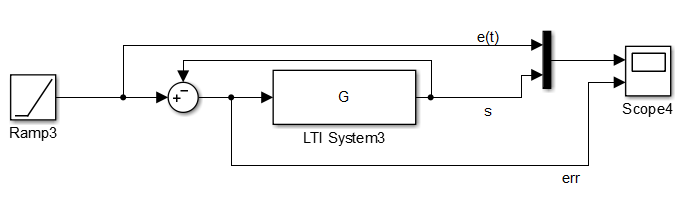
\includegraphics[scale=0.5]{sim1.png}
	\captionof{figure}{\textit{Schema SIMULINK de la boucle fermée \\}}
	\label{fig1} 
	\end{center}   
\chapter{\textsc{Analyse du procédé un bac d'eau}}
\section{\textsc{Le procédé}}
 
\chapter{\textsc{Echantillonnage du signal d'erreur }}
\section{\textsc{La plage de valeurs de $T_e$}}

\par Pour déterminer cette plage de valeurs on doit calculer les valeurs propres du système de la boucle d'asservissement vu précédemment. Les pôles calculés par MATLAB valent :$ 
   \left \{
   \begin{array}{r c l}
      p_1  & = & -8.8730 \\
      p_2 & = & -1.1270
   \end{array}
   \right .$ 
   On prend le pôle dominant soit $p_2$  et :
   
   \begin{center}
   		$\frac{1}{|p_2|}<T_e<|p_2| \Rightarrow  0.28175 <T_e< 1.127 $
   \end{center}
  
\section{\textsc{Vérification de l'analyse avec MATLAB/SIMULINK}}

\subsection{Visualisation}

\begin{center}
	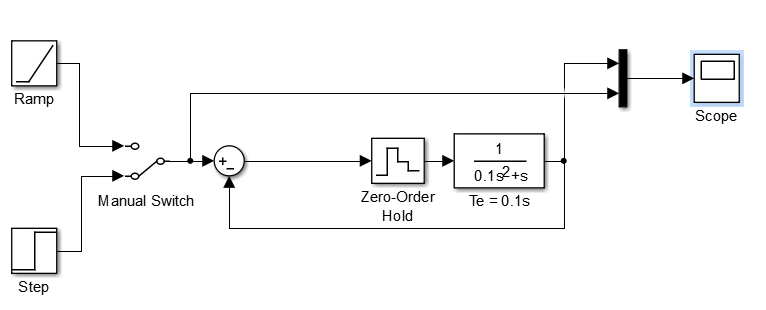
\includegraphics[scale=0.5]{shem11.png}
	\captionof{figure}{\textit{Schema simulink du système échantillonné pour différentes valeurs de $T_e$ \\}}
	\label{fig8} 
	\end{center}
	
	\begin{center}
	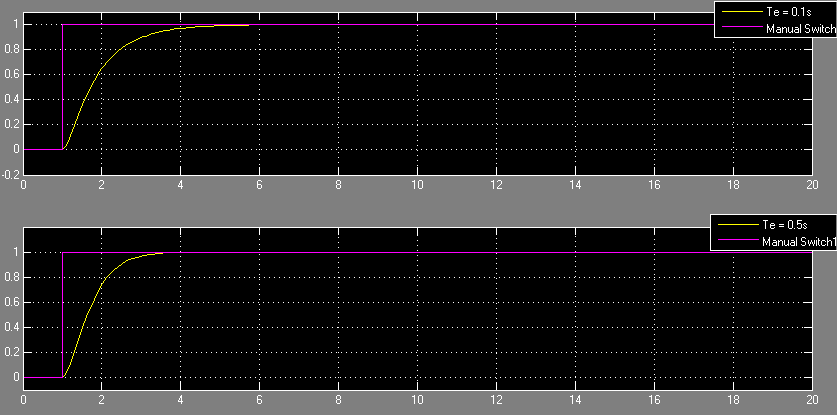
\includegraphics[scale=0.4]{simu11.png}
	\captionof{figure}{\textit{Réponses simulink de $s(t)$ pour de $T_e=0.1s$ et $T_e=0.5s$ \\}}
	\label{fig9} 
	\end{center}
	
	\begin{center}
	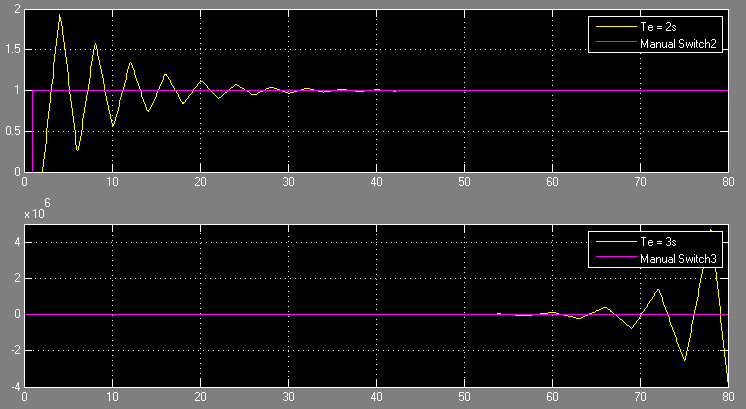
\includegraphics[scale=0.5]{simu22.png}
	\captionof{figure}{\textit{Réponses simulink de $s(t)$ pour de $T_e=2s$ et $T_e=3s$ \\}}
	\label{fig10} 
	\end{center}

\subsection{Commentaires}

\par Le système asservi diverge pour $T_e = 3 s$,  pour $T_e = 2 s$ il possède plusieurs oscillations et tarde à converger donc ces deux cas seront écartés.\\

   	
%	\begin{center}
%	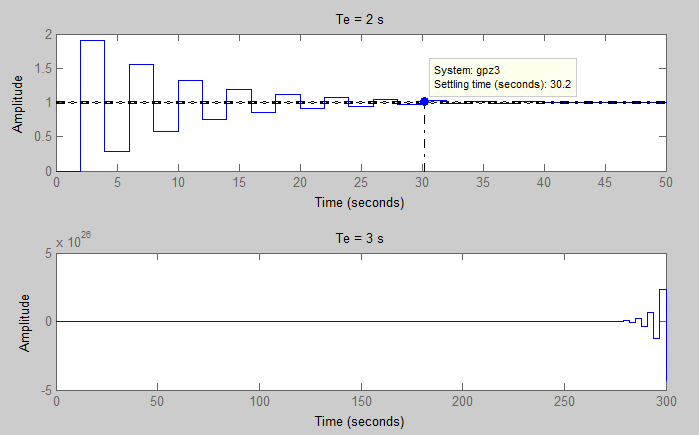
\includegraphics[scale=0.5]{mat2.png}
%	\captionof{figure}{\textit{Réponses $s(t)$ pour de $T_e=2s$ et $T_e=3s$ \\}}
%	\label{fig7} 
%	\end{center}

Il nous reste à comparer entre la réponse à $T_e=0.1s$ et à  $T_e=0.5s$, comparons leurs temps de réponses respectifs:\\
   
   	
%	\begin{center}
%	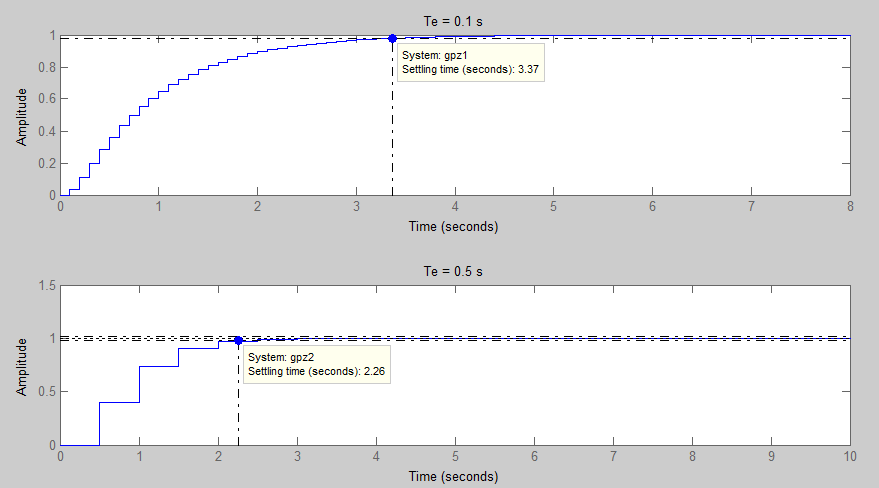
\includegraphics[scale=0.5]{mat1.png}
%	\captionof{figure}{\textit{Réponses $s(t)$ pour de $T_e=0.1s$ et $T_e=0.5s$ \\}}
%	\label{fig8} 
%	\end{center}
	
\par Il est clair qu'on écartera l'échantillonnge à $T_e=0.1$ et on retiendra celui à $T_e=0.5$ car le premier possède un temps de réponse $t_r=3.6113s$, il est plus grand que le temps de réponse que possède le système en temps continu contrairement à l'échantillonnage à $T_e=0.5 $ qui possède un temps de réponse $t_r = 2.8161 s$ et ne possède pas de dépassement,alors il respecte toutes les performances du système en temps continu.\\ 	
	

\textbf{Nota :} \label{section 2.2.2} \hyperref[Annexe A]{voir Annexe A} pour une analyse du système asservi discrétisé avec la commande MATLAB "c2d" et sur SIMULINK en utilisant le bloc LTI. On remarquera que le système asservi discrétisé garde les mêmes dynamiques que le système asservi echantillonné vu en dessus.

\section{\textsc{Visualisation de $s(t)$ pour la consigne $e_{ref}$}}

	\begin{center}
	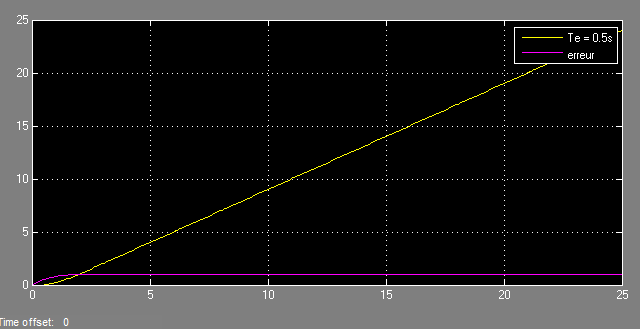
\includegraphics[scale=0.5]{simu3.png}
	\captionof{figure}{\textit{Réponse Simulink $s(t)$ à $T_e=0.5s$ en jaune pour la consigne $e_{ref}=e_1t$ et l'erreur $\epsilon (t) $ en mauve. \\}}
	\label{fig11} 
	\end{center}

\textbf{Conclusion:L'erreur de traînage vaut toujours $e_1$}

\section{\textsc{La démonstration}}
\par En se servant du tableau des transformées en Z on obtient :

\begin{center}
	
$\overline{B_0G}(z^{-1}) = \frac{( \tau - e^{\frac{-T_e}{\tau}}-\tau + T_e )z^{-1} ( 1 + \frac{\tau - ( \tau - T_e ) e^{\frac{-T_e}{\tau}}}{\tau - e^{\frac{-T_e}{\tau}}-\tau + T_e} ) z^{-1}} {(1-z^{-1}) (1- ( e^{\frac{-T_e}{\tau}} ) z^{-1})}$\\[0.25 cm]
	
	$ \Rightarrow \left \{
   \begin{array}{r c l}
      a_1  = \tau - e^{\frac{-T_e}{\tau}}-\tau + T_e \\\\
      a_2 =  \frac{\tau - ( \tau - T_e ) e^{\frac{-T_e}{\tau}}}{\tau - e^{\frac{-T_e}{\tau}}-\tau + T_e} \\\\
      b_1 = e^{\frac{-T_e}{\tau}}
   \end{array}
   \right . $
			
\end{center}


\par Ce qu'on va faire c'est de transformer $\overline{B_0G}(z^{-1})$ en $\overline{B_0G}(z)$ et ensuite l'identifier avec la fonction de transfert $G(p)$ discrétisée sous MATLAB avec la commande "c2d" et qu'on appelera $Gz(z)$, nous obtenons:

	\begin{center}
	 		
			$\overline{B_0G}(z)= \frac{a_1 z + a_1a_2}{z^2 -(b_1+1)z-b_1} $ \\[0.25cm]
			$Gz(z)= \frac{0.4007 z+ 0.09596}{z^2 + 1.007 z+ 0.006738} $\\[0.25cm]
			L'identification nous donne les valeurs numériques suivantes : $\Rightarrow 
	 \left \{
   \begin{array}{r c l}
      a_1 = 0.4007 \\
      a_2 =   0.3395\\
      b_1 = 0.00674
   \end{array}
   \right . $
	\end{center}
  
  \section{\textsc{Analyse de la stabilité par le lieu des racines}}
  
\par En utilisant cette méthode on pourra facilement en déduire le domaine de stabilité du système asservi. On utilisera pour ça la commande MATLAB "rltool":

	\begin{center}
	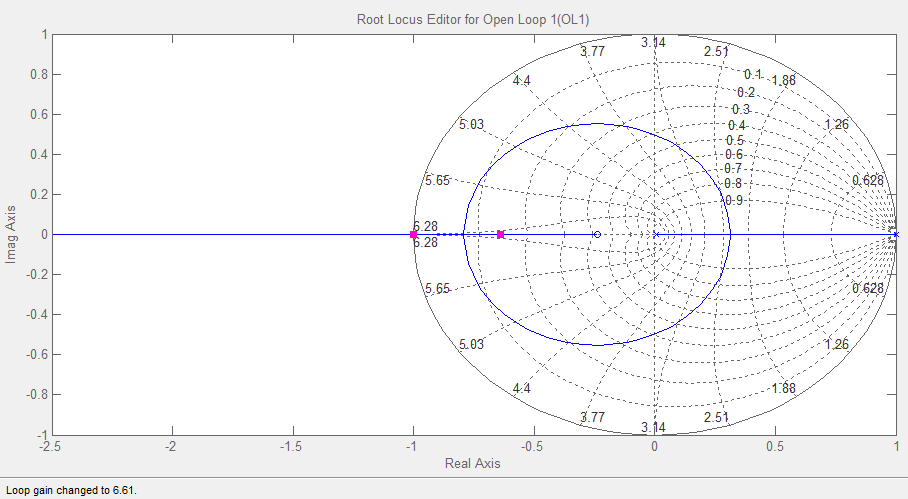
\includegraphics[scale=0.4]{rltool1.png}
	\captionof{figure}{\textit{ Le lieu des racines de la boucle fermée.\\}} 
	\label{fig12} 
	\end{center}

\par Puisque les deux pôles sont situé à l'intérieur du cercle unité alors le système asservi est asymptotiquement stable, de plus comme le montre la figure ci-dessus la stabilité est dissoute en appliquant un correcteur proprtionnel qui vaut plus de $ 6.61 $ cela explique que le domaine de stabilité du système bouclé est comprise entre :$K_p \in ]0,6.61]$.

%\section{\textsc{Calcul théorique de l'erreur de traînage $\epsilon_v$}}


\chapter{\textsc{Introdution d'une correction numérique }}
\section{\textsc{L'effet du temps de conversion et les temps d'exécution}}

\par Lorsque le temps de conversion A/N, N/A et les temps d'exécution seront négligés, la période d'échantillonnage calculée ne sera pas éronnée.\\

   \section{\textsc{L'effet du temps de conversion et les temps d'exécution}}
   
   \par Le rôle du pôle $z=1$ du correcteur $C_1(z^{-1}$ est d'éliminner l'eereur de traînage. Celui du zéro $b_1$ est d'éliminer le rôle du pôle $z=b_1$ de $B_0G(z^{-1})$. Le rôle du pôle $z=-a_2$ est d'éliminer l'effet du zéro $z=-a_2$ de $B_0G(z^{-1})$. Enfin le rôle du zéro $a$ est d'éliminer l'effet du pôle $z=1$.\\[0.5 cm]
   \par a doit être comprise entre 0 et 1 pour des raisons de stabilité.
   
   \section{\textsc{Visualisation de $s(t)$ pour différentes valeurs de $a$}}
   
   	\begin{center}
	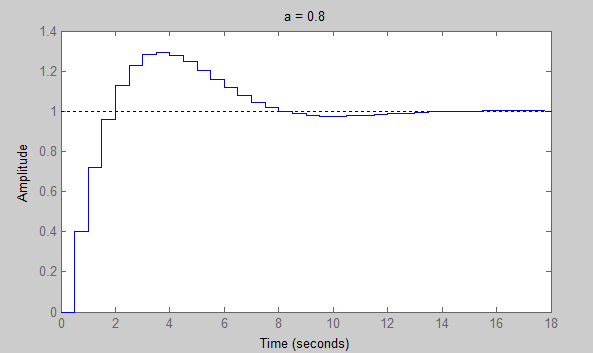
\includegraphics[scale=0.5]{a8.png}
	\captionof{figure}{\textit{Tracé de la sortie  $ s(t) $ pour $a=0.8$. \\}}
	\label{fig13} 
	\end{center}
	
		\begin{center}
	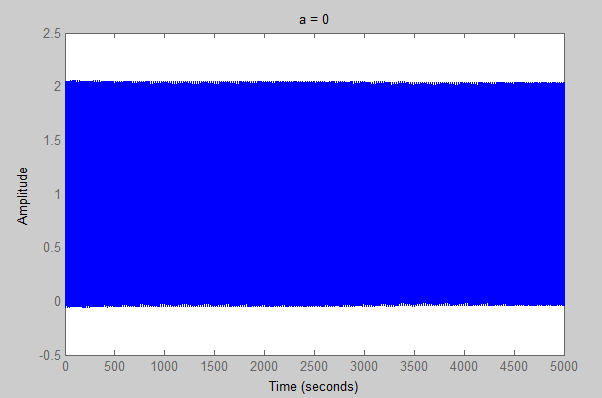
\includegraphics[scale=0.5]{a0.png}
	\captionof{figure}{\textit{Tracé de la sortie  $ s(t) $ pour $a=0$. \\}}
	\label{fig14} 
	\end{center}
	
		\begin{center}
	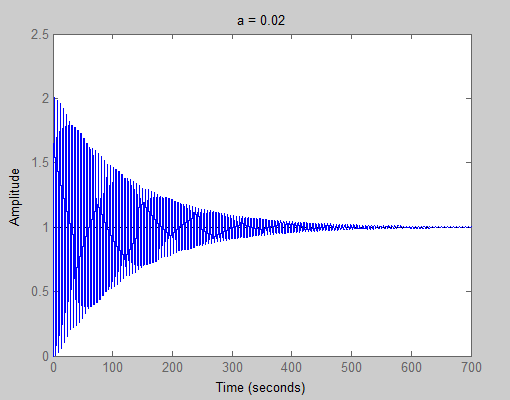
\includegraphics[scale=0.5]{a2.png}
	\captionof{figure}{\textit{Tracé de la sortie  $ s(t) $ pour $a=0.02$. \\}}
	\label{fig15} 
	\end{center}
 	
 		\par Il est clair qu'on choisira $a=0.8$ car c'est la seule valeur ou le système converge.
 		
 \section{\textsc{Stabilité du système en boucle ouverte avec correcteur par les lieux des racines pour différentes valeurs de $a$}}
 
 		\begin{center}
	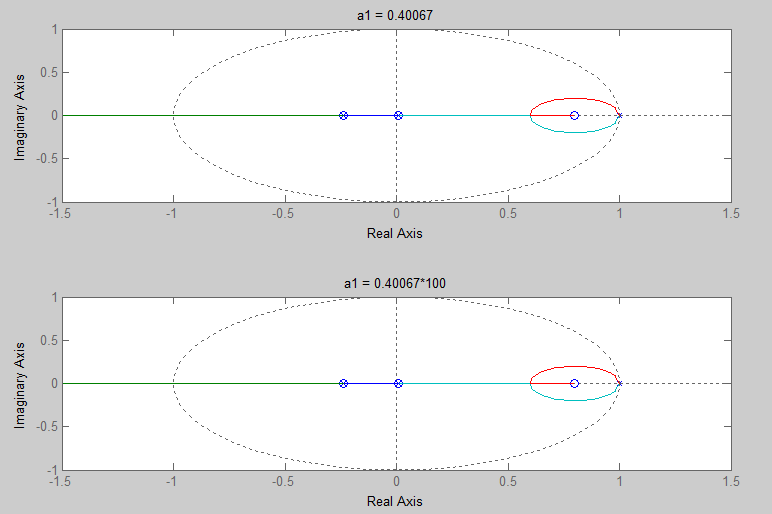
\includegraphics[scale=0.5]{rl3.png}
	\captionof{figure}{\textit{Rlocus pour $a1=0.4007$ et pour $a1=4.007$ . \\}}
	\label{fig17} 
	\end{center}
		
	\par Même pour une valeur de $a_1$ dix fois plus grande, la stabilité du système n'est pas affectée. Tous les pôles sont à l'intérieur du disque unité.
  	
\chapter*{\textsc{Conclusion}}
\addcontentsline{toc}{chapter}{\textsc{Conclusion}}
  
  \par A défaut de temps nous n'avons pas pu finir les parties restantes de cette séance de TP. On tient à s'excuser auprès de M Gouaisbaut et de M Fergani.
%\input{conclusion.tex}

\begin{appendices}

\chapter*{\textsc{Annexe A}}
	\addcontentsline{toc}{chapter}{\textsc{Annexe A}}		
	
	\label{Annexe A} \hyperref[section 2.2.2]{Retour vers section 2.2.2}
	
	\subsection{Visualisation}

	\begin{center}
	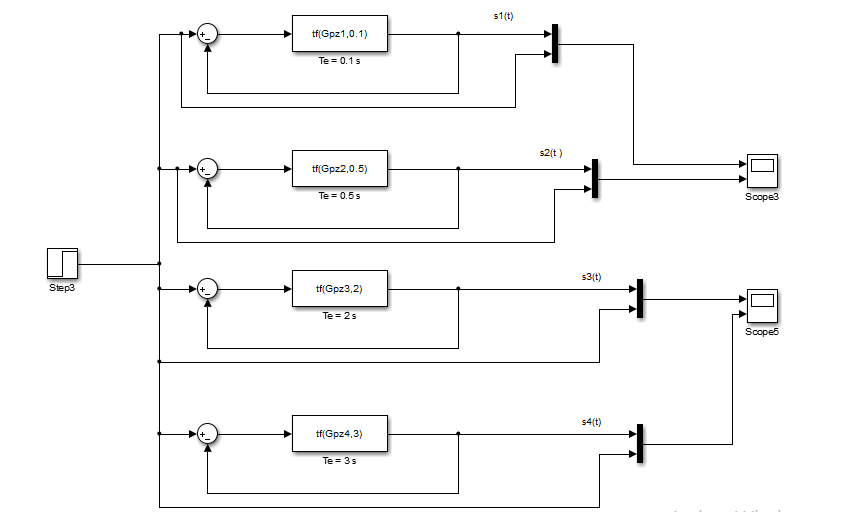
\includegraphics[scale=0.5]{shem1.png}
	\captionof{figure}{\textit{Schema simulink du système échantillonné pour différentes valeurs de $T_e$ \\}}
	\label{fig4} 
	\end{center}
	
	\begin{center}
	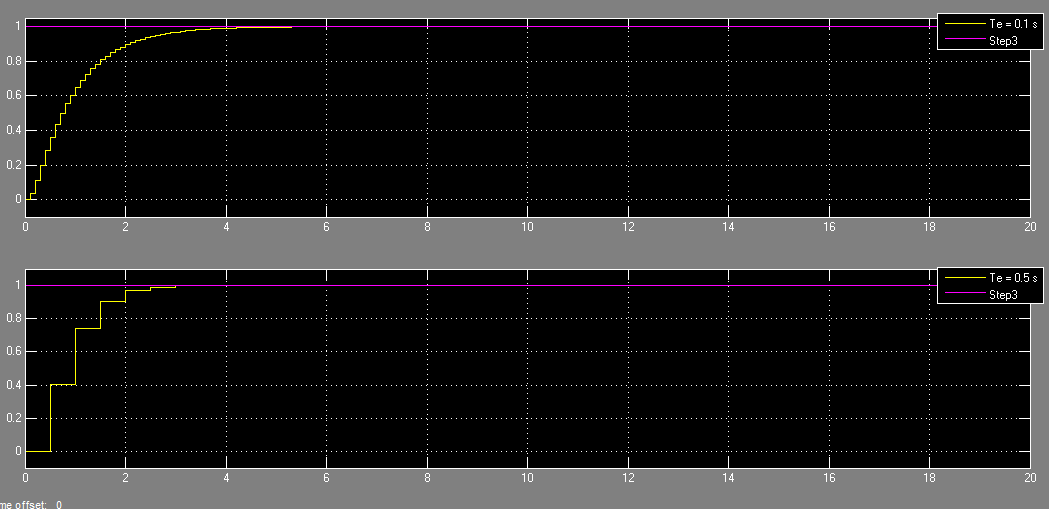
\includegraphics[scale=0.4]{simu1.png}
	\captionof{figure}{\textit{Réponses simulink de $s(t)$ pour de $T_e=0.1s$ et $T_e=0.5s$ \\}}
	\label{fig5} 
	\end{center}
	
	\begin{center}
	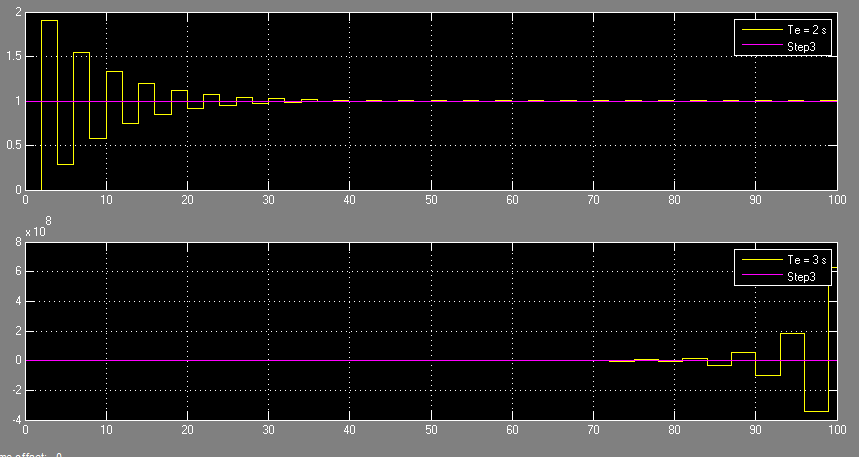
\includegraphics[scale=0.5]{simu2.png}
	\captionof{figure}{\textit{Réponses simulink de $s(t)$ pour de $T_e=2s$ et $T_e=3s$ \\}}
	\label{fig6} 
	\end{center}
	
\subsection{Commentaires}

\par Le système diverge pour $T_e = 3 s$, il possède plusieurs oscillations et tarde à ce converger pour $T_e = 2 s$ donc ces deux cas seront écartés.\\

   	
	\begin{center}
	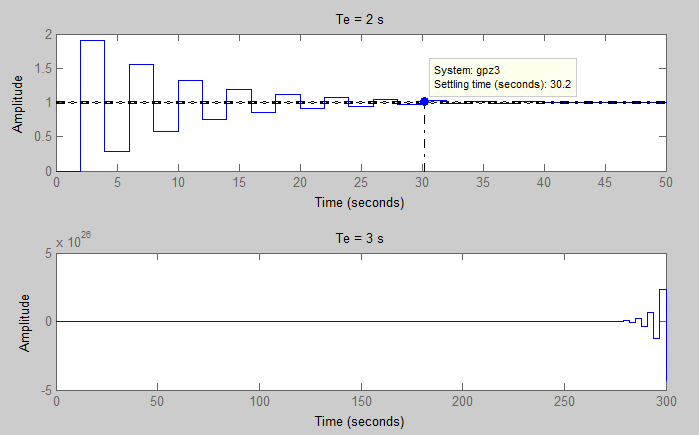
\includegraphics[scale=0.5]{mat2.png}
	\captionof{figure}{\textit{Réponses $s(t)$ pour de $T_e=2s$ et $T_e=3s$ \\}}
	\label{fig7} 
	\end{center}

Il nous reste à comparer entre la réponse à $T_e=0.1s$ et à  $T_e=0.5s$, comparons leurs temps de réponses respectifs:\\
   
   	
	\begin{center}
	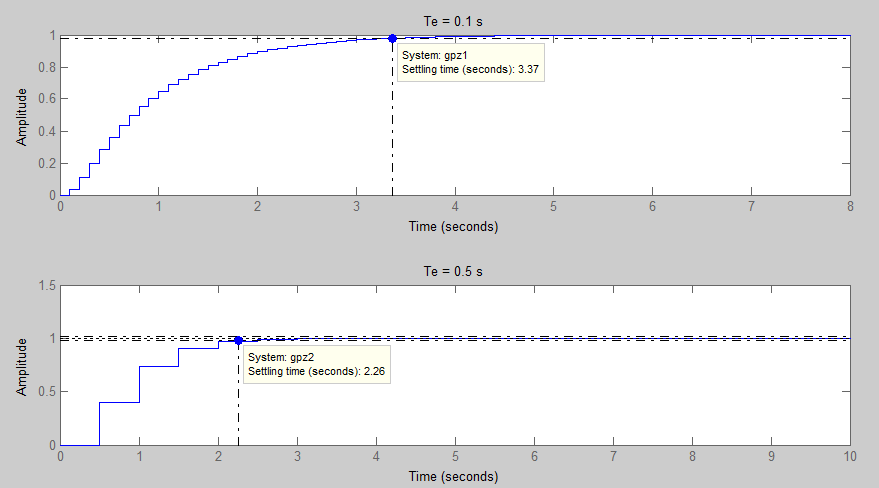
\includegraphics[scale=0.5]{mat1.png}
	\captionof{figure}{\textit{Réponses $s(t)$ pour de $T_e=0.1s$ et $T_e=0.5s$ \\}}
	\label{fig8} 
	\end{center}
	
\par Il est clair qu'on écartera l'échantillonnge à $T_e=0.1$ et on retiendra celui à $T_e=0.5$ car le premier ne respecte pas le temps de réponse que possède le système en temps continu contrairement à l'échantillonnage à $T_e=0.5 $ qui possède un temps de réponse $t_r = 2.26 s$ et ne possède pas de dépassement,alors il respecte toutes les performances du système en temps continu.\\ 	

\chapter*{\textsc{Annexe B}}
	\addcontentsline{toc}{chapter}{\textsc{Annexe B}}	
	\par Code Matlab.\\
	\begin{lstlisting}
	
clc
clear all
close all
t=0.1;
Kg=1;
G=tf([Kg],[t 1 0]);


Gbf=feedback(G,1);

% figure(1)
% margin(G)
% grid
% 
% figure(2)
% step(Gbf)
%   
% margin(Gbf)
% grid
T=feedback(G,1);
S=1-T;
pole(T)



Gpz1=c2d(G,0.1,'zoh')
gpz1=feedback(Gpz1,1);
% 
Gpz2=c2d(G,0.5,'zoh')
gpz2=feedback(Gpz2,1);
% 
Gpz3=c2d(G,2,'zoh')
gpz3=feedback(Gpz3,1);
 
Gpz4=c2d(G,3,'zoh')
gpz4=feedback(Gpz4,1);


figure(3)
subplot(2,1,1)
step(gpz1 )
title('Te = 0.1 s')

subplot(2,1,2)
step(gpz2)
title('Te = 0.5 s')


figure(4)
subplot(2,1,1)
step(gpz3)
title('Te = 2 s')

subplot(2,1,2)
step(gpz4)
title('Te = 3 s')


%rltool(Gpz2)

figure(5)
eig(feedback(6.60775*Gpz2,1))
eig(feedback(0.000000000000000000000000001*Gpz2,1))
%pour Te=0.5
b1=0.006738;
a1=0.40067;
a=0.8;
%a0=0;
%a=0.02;
a2=0.2395;
C1=zpk([a b1],[1 -a2],[1],0.5);
Bo=C1*Gpz2;
BoBF=feedback(Bo,1);
step(BoBF)
title('a = 0.8')

figure(6)
subplot(2,1,1)
rlocus(Bo)
title('a1 = 0.40067')
subplot(2,1,2)
Bo1=C1*Gpz2*100;
rlocus(Bo1)
title('a1 = 0.40067*100')
	
	\end{lstlisting}
	
\end{appendices}	
%*********************** Bibliographie ************ 
\bibliographystyle{alpha}
\bibliography{biblio}  



\end{document}